\documentclass[a4paper,12pt]{article}
\usepackage[utf8]{inputenc}
\usepackage{cmap}
\usepackage[T2A]{fontenc}
\usepackage{textcomp}
\usepackage[russian]{babel}
\usepackage{url}
\usepackage{graphicx}
\usepackage{float}
\usepackage{booktabs}
\usepackage{enumitem}
\usepackage{soulutf8}

\usepackage{parskip}

\usepackage{emptypage}
\usepackage{subcaption}
\usepackage{multicol}
\usepackage{xcolor}

% Math stuff
\usepackage{amsmath, amsfonts, mathtools, amsthm, amssymb}
% Fancy script capitals
\usepackage{mathrsfs}
\usepackage{cancel}
% Bold math
\usepackage{bm}
% Some shortcuts
\newcommand\N{\ensuremath{\mathbb{N}}}
\newcommand\R{\ensuremath{\mathbb{R}}}
\newcommand\Z{\ensuremath{\mathbb{Z}}}
\renewcommand\O{\ensuremath{\emptyset}}
\newcommand\Q{\ensuremath{\mathbb{Q}}}
\renewcommand\C{\ensuremath{\mathbb{C}}}

%Make implies and impliedby shorter
\let\implies\Rightarrow
\let\impliedby\Leftarrow
\let\iff\Leftrightarrow
\let\epsilon\varepsilon

\usepackage{mdframed}
\mdfsetup{skipabove=1em,skipbelow=0em}

\newmdtheoremenv[nobreak=true]{theorem}{Теорема}[section]
\newmdtheoremenv[nobreak=true]{corollary}{Следствие}[theorem]
\newmdtheoremenv[nobreak=true]{lemma}[theorem]{Лемма}

\theoremstyle{remark}
\newtheorem*{remark}{Утверждение}

\theoremstyle{definition}
\newmdtheoremenv[nobreak=true]{definition}{Определение}[section]

\renewcommand\qedsymbol{$\blacksquare$}

\makeatletter
\def\thm@space@setup{%
  \thm@preskip=\parskip \thm@postskip=0pt
}

\usepackage{xifthen}


\def\@lecture{}%
\newcommand{\lecture}[2]{
    \ifthenelse{\isempty{#2}}{%
        \def\@lecture{Лекция #1}%
    }{%
        \def\@lecture{Лекция #1: #2}%
    }%
    \section{\@lecture}
}

\usepackage{geometry}  
\geometry{left=20mm,right=20mm,top=25mm,bottom=30mm} % задание полей текста
\setlength{\headheight}{18pt}
\usepackage{fancyhdr}
\pagestyle{fancy}
\renewcommand{\footrulewidth}{0.4pt}

% LE: left even
% RO: right odd
% CE, CO: center even, center odd

\fancyhead[RO,LE]{} % Right odd,  Left even
\fancyhead[RE,LO]{\@lecture}          % Right even, Left odd

\fancyfoot[RO,LE]{\thepage}  % Right odd,  Left even
\fancyfoot[RE,LO]{\CourseInfo}          % Right even, Left odd
\fancyfoot[C]{}

\makeatother

\usepackage{hyperref}
\usepackage{xcolor}
\hypersetup{			
	unicode=true,           
	pdfstartview=FitH,
	colorlinks=true,       	
	linkcolor=blue,         
	citecolor=green,        
	filecolor=magenta,      
	urlcolor=cyan,          
}

\usepackage{tcolorbox}

\usepackage{listings}
\lstset{ 
  backgroundcolor=\color{white},   % цвет фона
  basicstyle=\footnotesize,        % размер
  breakatwhitespace=false,         % проблемы с отступами
  breaklines=true,                 % автоматический переход на новую строку
  captionpos=b,                    % sets the caption-position to bottom
  commentstyle=\color{black},      % стиль комментариев
  escapeinside={\%*}{*)},          % для вставки латеха в код
  frame=single,	                   % рамочка вокруг
  keepspaces=true,                 % сохраняет пробелы в коде (чтобы был кодстайл)
  keywordstyle=\color{blue},       % стиль кода
  language=C++,                    % язык программирования!
  morekeywords={*,...},            % увеличение словаря
  numbers=left,                    % где будет нумерация строк (none, left, right)
  numbersep=8pt,                   % расстояние между нумерацией и кодом
  numberstyle=\color{gray},        % стиль нумерации
  rulecolor=\color{gray},          % цвет рамки
  showspaces=false,                % если тру, то заменяет пробелы на особые подчеркивания; конфликтует с 'showstringspaces'
  showstringspaces=false,          % особые подчеркивания вместо пробелов в строках
  showtabs=false,                  % подчеркивания вместо табов
  stepnumber=1,                    % как часто показывать нумерацию. Если 1, то нумеруется каждая строка
  stringstyle=\color{violet},      % цвет строк
  tabsize=2,	                       % дефолтный размер таба
  texcl=true,
  title=\lstname                   % вставляет название файла, если импорт
}

\makeatletter
\newcommand{\highlight}[1]{%
  \setbox\@tempboxa\hbox{#1}%
  \ifdim\wd\@tempboxa>\linewidth
    \noindent
    \colorbox{pink}{%
      \parbox{\dimexpr\linewidth-2\fboxsep}{#1}%
    }%
  \else
    \colorbox{pink}{#1}%
  \fi}%Highlighter.
\makeatother

\newcommand{\CourseInfo}{Курсовая работа по курсу <<Базы данных>>}

\begin{document}
\title{\CourseInfo}
\author{Евсюков Никита Александрович \\ Б05-911}
\date{База данных <<Система анализа электропотребления>>}
\maketitle

\section{Концептуальная модель}

\begin{figure}[H]    
  \centering    
  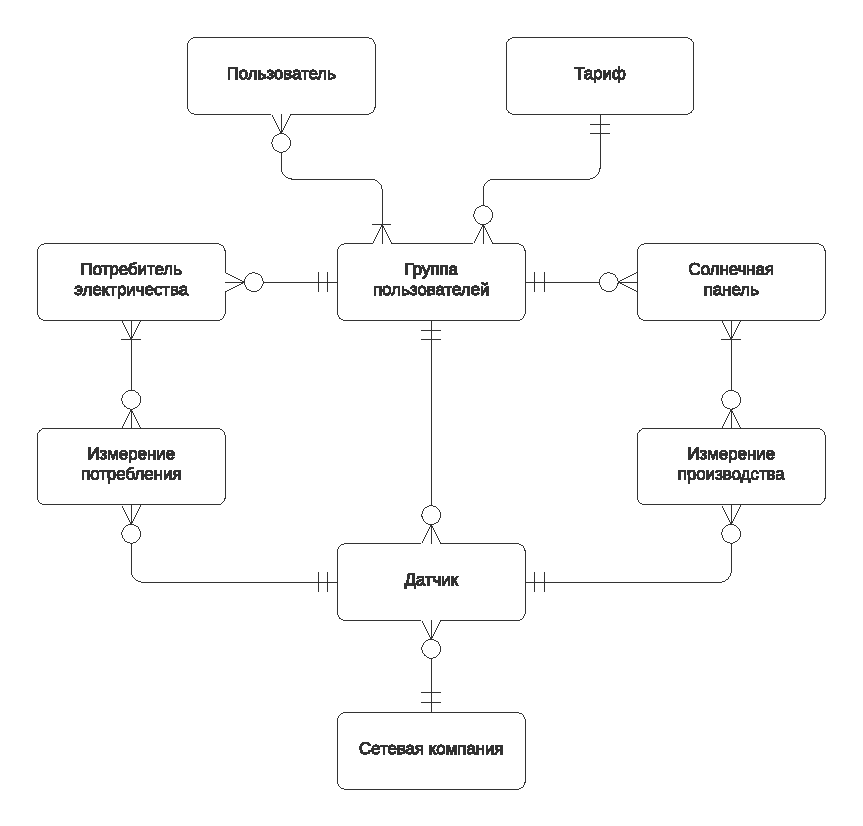
\includegraphics[width=0.8\textwidth]{include/concept.pdf}    
  \caption{Концептуальная модель}        
  \label{flg:scheme1}    
\end{figure} 

\section{Логическая модель}

\begin{figure}[H]    
  \centering    
  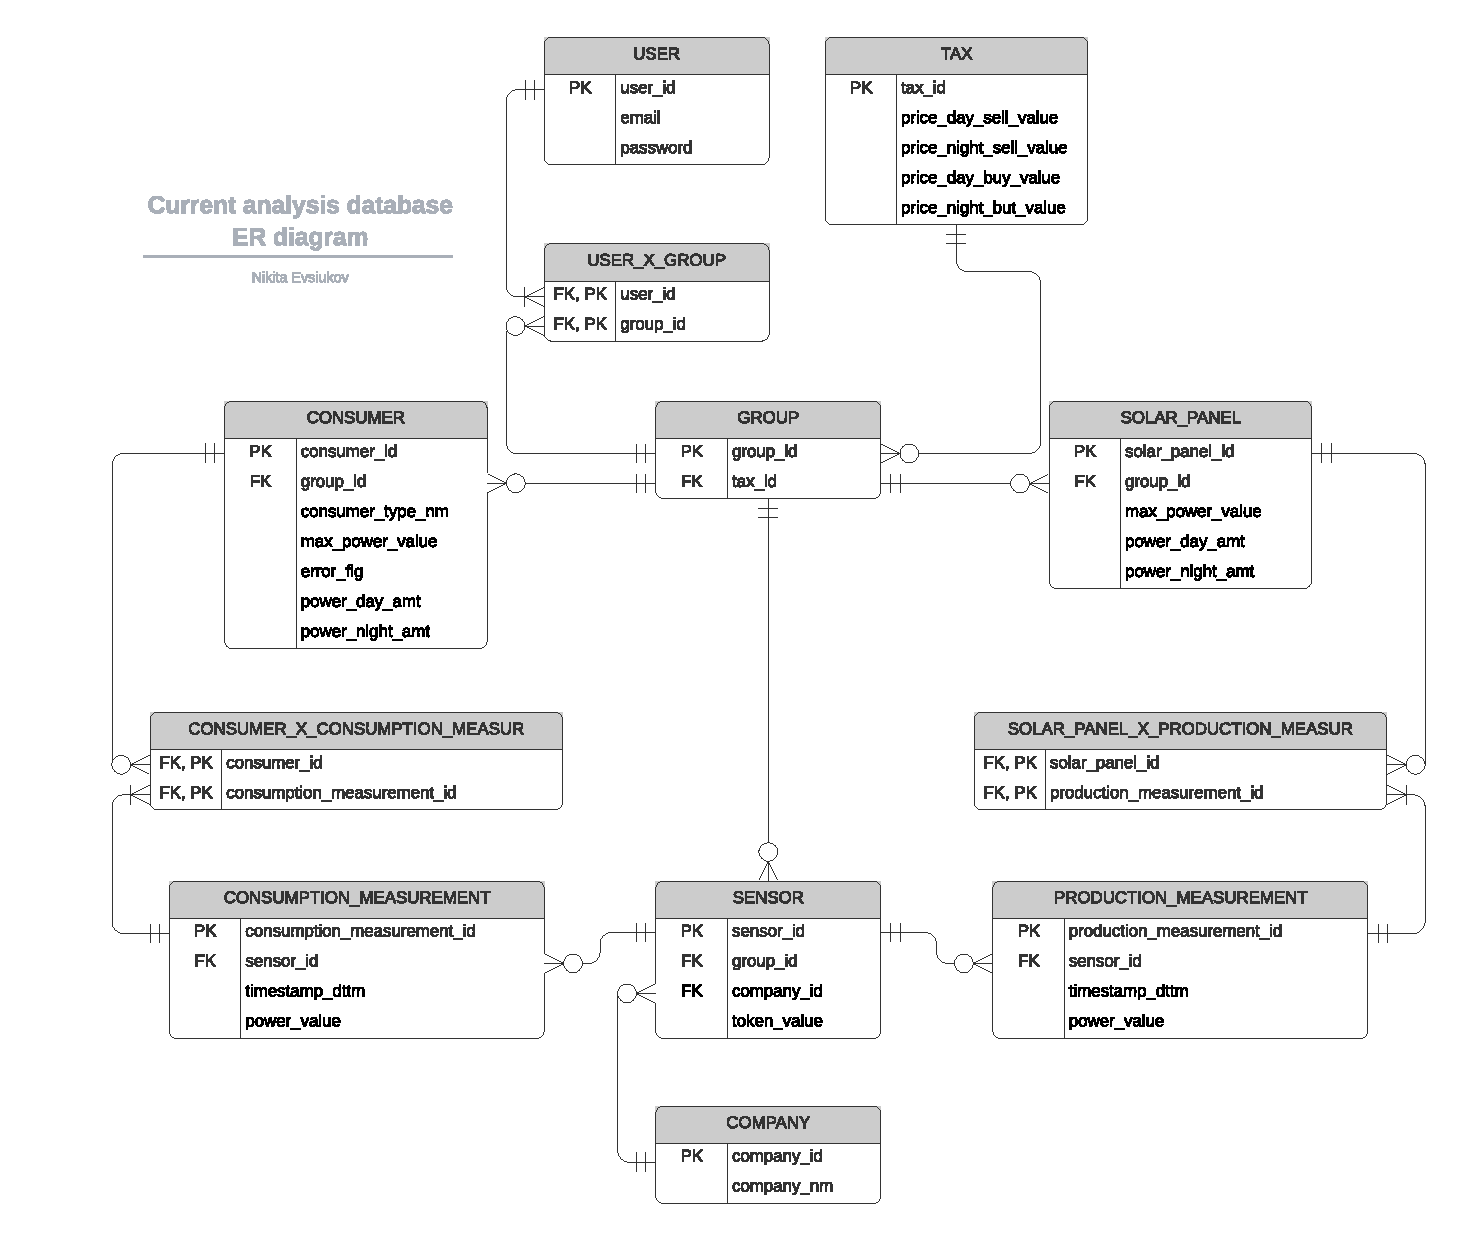
\includegraphics[width=1.0\textwidth]{include/logic.pdf}    
  \caption{Логическая модель}        
  \label{flg:scheme2}    
\end{figure} 

\newpage
\section{Физическая модель}

\begin{table}[H]
\begin{tabular}{|l|l|l|l|}
\hline
\multicolumn{4}{|l|}{USER / Пользователь}                                                                           \\ \hline
Название & Описание                   & Тип данных & Ограничени                                                     \\ \hline
user\_id & ID пользователя            & SERIAL     & \begin{tabular}[c]{@{}l@{}}PRIMARY KEY\end{tabular} \\ \hline
email    & Email пользователя         & TEXT       & \begin{tabular}[c]{@{}l@{}}NOT NULL\\ UNIQUE\end{tabular}      \\ \hline
password & Хеш от пароля пользователя & TEXT       & NOT NULL                                                       \\ \hline
\end{tabular}
\end{table}

\begin{table}[H]
\begin{tabular}{|l|l|l|l|}
\hline
\multicolumn{4}{|l|}{USER\_X\_GROUP / Пользователи в группах}                                                \\ \hline
Название  & Описание        & Тип данных & Ограничени                                                        \\ \hline
user\_id  & ID пользователя & SERIAL     & \begin{tabular}[c]{@{}l@{}}PRIMARY KEY\\ FOREIGN KEY\end{tabular} \\ \hline
group\_id & ID группы       & SERIAL     & \begin{tabular}[c]{@{}l@{}}PRIMARY KEY\\ FOREIGN KEY\end{tabular} \\ \hline
\end{tabular}
\end{table}

\begin{table}[H]
\begin{tabular}{|l|l|l|l|}
\hline
\multicolumn{4}{|l|}{GROUP  /  Группа пользователей}               \\ \hline
Название  & Описание                    & Тип данных & Ограничени  \\ \hline
group\_id & ID группы пользователей     & SERIAL     & PRIMARY KEY \\ \hline
tax\_id  & ID тарифа на электроэнергию & SERIAL     & FOREIGN KEY \\ \hline
\end{tabular}
\end{table}

\begin{table}[H]
\begin{tabular}{|l|l|l|l|}
\hline
\multicolumn{4}{|l|}{TAX  /  Тарифы на электроэнергию}                                                                                          \\ \hline
Название                  & Описание                                                                              & Тип данных     & Ограничени  \\ \hline
tax\_id                  & ID тарифа                                                                             & SERIAL         & PRIMARY KEY \\ \hline
price\_day\_sell\_value   & \begin{tabular}[c]{@{}l@{}}Цена продажи \\ электроэнергии днём за КВт*ч\end{tabular}  & NUMERIC(10, 2) &             \\ \hline
price\_night\_sell\_value & \begin{tabular}[c]{@{}l@{}}Цена продажи \\ электроэнергии ночью за КВт*ч\end{tabular} & NUMERIC(10, 2) &             \\ \hline
price\_day\_buy\_value    & \begin{tabular}[c]{@{}l@{}}Цена покупки \\ электроэнергии днём за КВт*ч\end{tabular}  & NUMERIC(10, 2) &             \\ \hline
price\_night\_buy\_value  & \begin{tabular}[c]{@{}l@{}}Цена покупки \\ электроэнергии ночью КВт*ч\end{tabular}    & NUMERIC(10, 2) &             \\ \hline
\end{tabular}
\end{table}

\begin{table}[H]
\begin{tabular}{|l|l|l|l|}
\hline
\multicolumn{4}{|l|}{CONSUMER  /  Потребитель электроэнергии}                                                                                                     \\ \hline
Название           & Описание                                                                                                      & Тип данных     & Ограничени  \\ \hline
consumer\_id       & ID потребителя                                                                                                & SERIAL         & PRIMARY KEY \\ \hline
group\_id          & \begin{tabular}[c]{@{}l@{}}ID группы, которой принадлежит\\ потребитель\end{tabular}                          & SERIAL         & FOREIGN KEY \\ \hline
consumer\_type\_nm & \begin{tabular}[c]{@{}l@{}}Название типа потребителя,\\ например, "чайник"\end{tabular}                       & TEXT           &             \\ \hline
max\_power\_value  & \begin{tabular}[c]{@{}l@{}}Максимальная нагрузка \\ потребителя в Вт\end{tabular}                             & NUMERIC(20, 2)        &             \\ \hline
error\_flg         & \begin{tabular}[c]{@{}l@{}}Флаг, который показывает, что\\ устройство превысило лимит\\ нагрузки\end{tabular} & BOOLEAN        &             \\ \hline
power\_day\_amt    & \begin{tabular}[c]{@{}l@{}}Дневное суммарное потребление \\ в КВт*ч\end{tabular}                              & NUMERIC(20, 2) &             \\ \hline
power\_night\_amt  & \begin{tabular}[c]{@{}l@{}}Ночное суммарное потребление \\ в КВт*ч\end{tabular}                               & NUMERIC(20, 2) &             \\ \hline
\end{tabular}
\end{table}

\begin{table}[H]
\begin{tabular}{|l|l|l|l|}
\hline
\multicolumn{4}{|l|}{SOLAR\_PANEL  /  Солнечная панель}                                                                                      \\ \hline
Название          & Описание                                                                                  & Тип данных     & Ограничени  \\ \hline
solar\_panel\_id  & ID солнечной панели                                                                       & SERIAL         & PRIMARY KEY \\ \hline
group\_id         & \begin{tabular}[c]{@{}l@{}}ID группы, которой принадлежит\\ солнечная панель\end{tabular} & SERIAL         & FOREIGN KEY \\ \hline
max\_power\_value & \begin{tabular}[c]{@{}l@{}}Максимальная нагрузка \\ солнечной панели в Вт\end{tabular}    & NUMERIC(20, 2)        &             \\ \hline
power\_day\_amt   & \begin{tabular}[c]{@{}l@{}}Дневное суммарное производство \\ в КВт*ч\end{tabular}         & NUMERIC(20, 2) &             \\ \hline
power\_night\_amt & \begin{tabular}[c]{@{}l@{}}Ночное суммарное производство \\ в КВт*ч\end{tabular}          & NUMERIC(20, 2) &             \\ \hline
\end{tabular}
\end{table}

\begin{table}[H]
\begin{tabular}{|l|l|l|l|}
\hline
\multicolumn{4}{|l|}{CONSUMER\_X\_CONSUMPTION\_MEASUR  /  Потребители и их измерения}                                                   \\ \hline
Название                    & Описание                 & Тип данных & Ограничени                                                        \\ \hline
consumer\_id                & ID потребителя           & SERIAL     & \begin{tabular}[c]{@{}l@{}}PRIMARY KEY\\ FOREIGN KEY\end{tabular} \\ \hline
consumption\_masurement\_id & ID измерения потребления & SERIAL     & \begin{tabular}[c]{@{}l@{}}PRIMARY KEY\\ FOREIGN KEY\end{tabular} \\ \hline
\end{tabular}
\end{table}

\begin{table}[H]
\begin{tabular}{|l|l|l|l|}
\hline
\multicolumn{4}{|l|}{SOLAR\_PANEL\_X\_PRODUCTION\_MEASUR  /  Солнечные панели и их измерения}                                           \\ \hline
Название                   & Описание                  & Тип данных & Ограничени                                                        \\ \hline
solar\_panel\_id           & ID солнечной панели       & SERIAL     & \begin{tabular}[c]{@{}l@{}}PRIMARY KEY\\ FOREIGN KEY\end{tabular} \\ \hline
production\_masurement\_id & ID измерения производства & SERIAL     & \begin{tabular}[c]{@{}l@{}}PRIMARY KEY\\ FOREIGN KEY\end{tabular} \\ \hline
\end{tabular}
\end{table}

\begin{table}[H]
\begin{tabular}{|l|l|l|l|}
\hline
\multicolumn{4}{|l|}{CONSUMPTION\_MEASUREMENT  /  Измерение потребления}                                                                                                                       \\ \hline
Название                                                                & Описание                                                                              & Тип данных     & Ограничени  \\ \hline
\begin{tabular}[c]{@{}l@{}}consumption\_\\ measurement\_id\end{tabular} & ID измерения потребления                                                                   & SERIAL         & PRIMARY KEY \\ \hline
sensor\_id                                                              & \begin{tabular}[c]{@{}l@{}}ID датчика, которому \\ принадлежит измерение\end{tabular} & SERIAL         & FOREIGN KEY \\ \hline
timestamp\_dttm                                                         & Отметка времени измерения                                                             & TIMESTAMP(0)   &             \\ \hline
power\_value                                                            & Измеренная мощность в Вт                                                              & NUMERIC(20, 2) &             \\ \hline
\end{tabular}
\end{table}

\begin{table}[H]
\begin{tabular}{|l|l|l|l|}
\hline
\multicolumn{4}{|l|}{PRODUCTION\_MEASUREMENT  /  Измерение производства}                                                                                                                      \\ \hline
Название                                                               & Описание                                                                              & Тип данных     & Ограничени  \\ \hline
\begin{tabular}[c]{@{}l@{}}production\_\\ measurement\_id\end{tabular} & ID измерения производства                                                             & SERIAL         & PRIMARY KEY \\ \hline
sensor\_id                                                             & \begin{tabular}[c]{@{}l@{}}ID датчика, которому \\ принадлежит измерение\end{tabular} & SERIAL         & FOREIGN KEY \\ \hline
timestamp\_dttm                                                        & Отметка времени измерения                                                             & TIMESTAMP(0)   &             \\ \hline
power\_value                                                           & Измеренная мощность в Вт                                                              & NUMERIC(20, 2) &             \\ \hline
\end{tabular}
\end{table}

\begin{table}[H]
\begin{tabular}{|l|l|l|l|}
\hline
\multicolumn{4}{|l|}{SENSOR  /  Датчик}                                                                                                                                            \\ \hline
Название     & Описание                                                                                 & Тип данных & Ограничени                                                  \\ \hline
sensor\_id   & ID датчика                                                                               & SERIAL     & PRIMARY KEY                                                 \\ \hline
group\_id    & \begin{tabular}[c]{@{}l@{}}ID группы, которой\\ принадлежит датчик\end{tabular}          & SERIAL     & FOREIGN KEY                                                 \\ \hline
company\_id  & \begin{tabular}[c]{@{}l@{}}ID электрокомпании,\\ которая обслуживает датчик\end{tabular} & SERIAL     & FOREIGN KEY                                                 \\ \hline
token\_value & \begin{tabular}[c]{@{}l@{}}Уникальная\\ строка-идентификатор\\ датчика\end{tabular}      & TEXT       & \begin{tabular}[c]{@{}l@{}}NOT NULL, \\ UNIQUE\end{tabular} \\ \hline
\end{tabular}
\end{table}

\begin{table}[H]
\begin{tabular}{|l|l|l|l|}
\hline
\multicolumn{4}{|l|}{COMPANY  /  Электроэнергетическая компания} \\ \hline
Название      & Описание            & Тип данных  & Ограничени   \\ \hline
company\_id   & ID компании         & SERIAL      & PRIMARY KEY  \\ \hline
company\_nm   & Название компании   & TEXT        &              \\ \hline
\end{tabular}
\end{table}


\end{document}
